% Generated from tex/chapters/ch04/01_全体概要：この章で学ぶこと.tex for the SWEBOK structure tree
\subsection*{全体概要：この章で学ぶこと}
\addcontentsline{toc}{subsection}{全体概要：この章で学ぶこと}

この章は、ソフトウェアを実際に作る段階で必要になる知識を扱う。ここでいう「作る」とは、ソースコードを書くことだけではない。詳細設計を補い、テストし、部品を統合し、依存関係を管理し、性能を測り、運用に近い環境からのフィードバックを得ながら、ソフトウェアを完成度の高い形に近づけることである。

\noindent\textbf{到達目標}\quad この章を読み終えると、次のことができるようになる。

\begin{itemize}
  \item ソフトウェア構築が、設計、テスト、品質、構成管理、プロジェクト管理とどう関係するかを説明できる。
  \item 複雑さの最小化、変化への備え、検証しやすさ、再利用、標準適用の意味を説明できる。
  \item コーディング、単体テスト、統合、依存関係管理、継続的統合の実務上の役割を説明できる。
  \item API、例外処理、実行可能モデル、状態機械、ミドルウェア、クラウド、並行処理、性能調整などの構築技術を概観できる。
  \item 開発環境、単体テストツール、性能分析ツール、ローコード/ゼロコード環境の位置づけを説明できる。
\end{itemize}

\noindent\textbf{学習順序}\quad 初学者は、まず「構築とは何か」と「構築の基本原則」を押さえる。その後、「構築をどう管理するか」「現場で何を考えるか」「どの技術を使うか」「どのツールが支えるか」という順で読むとよい。

\begin{figure}[htbp]
\centering
\IfFileExists{assets/generated_figures/ch04/fig-ch04-01.png}{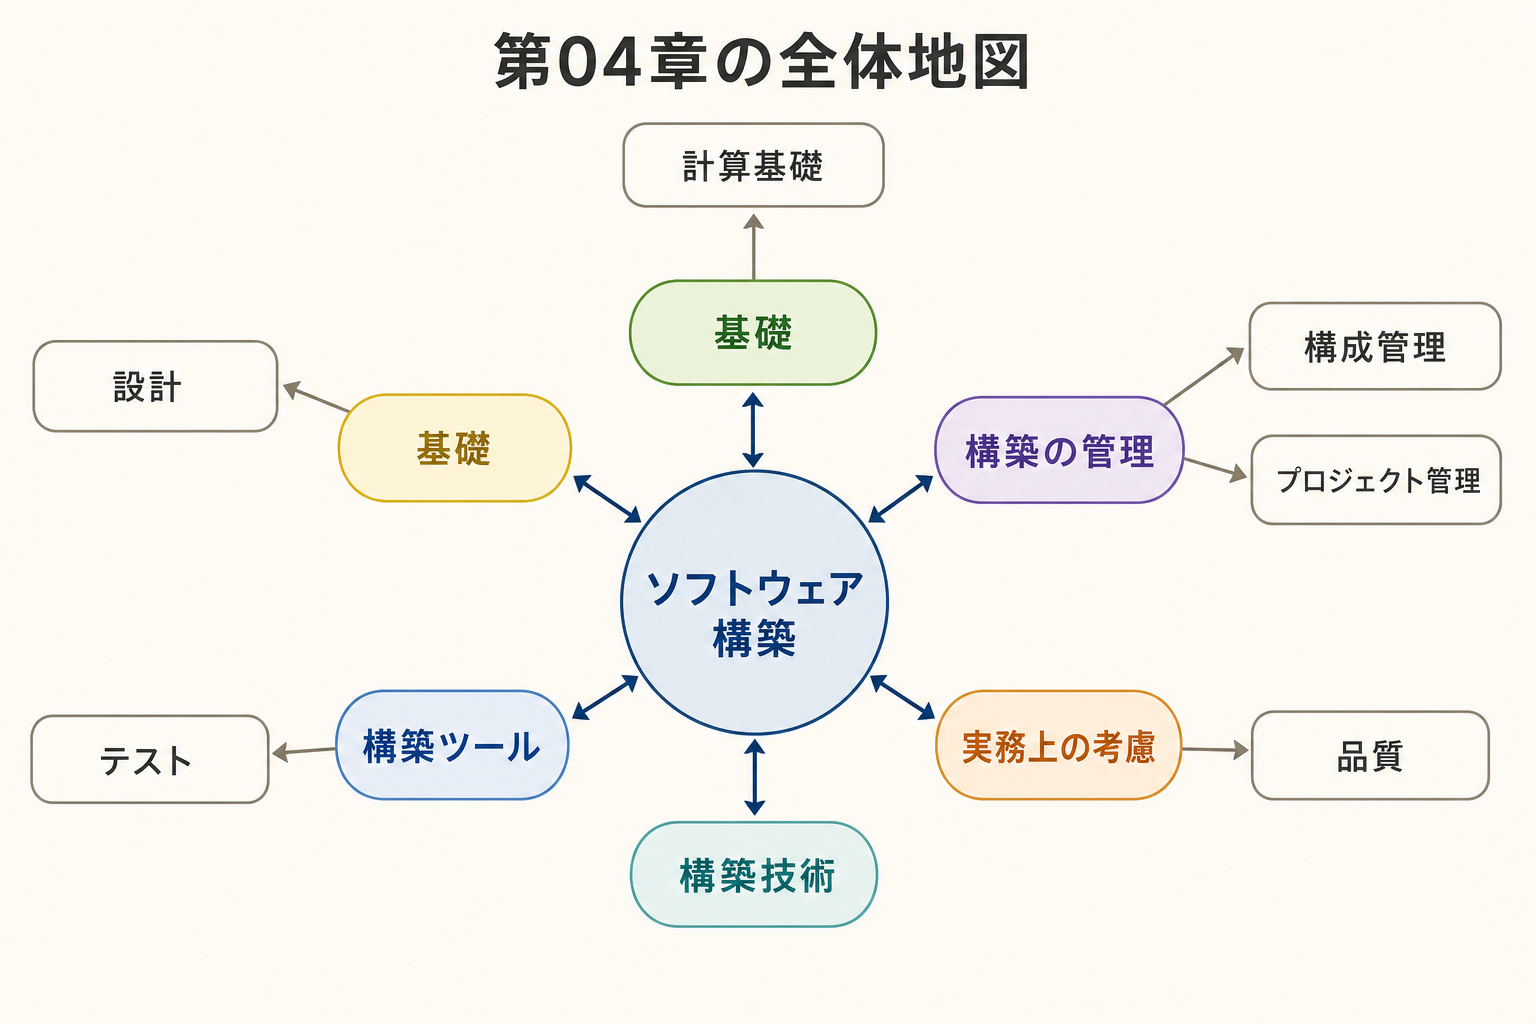
\includegraphics[width=0.96\linewidth]{assets/generated_figures/ch04/fig-ch04-01.png}}{\fbox{\parbox[c][48mm][c]{0.9\linewidth}{\centering 画像生成待ち\\第04章の全体地図}}}
\caption{第04章の全体地図}
\label{fig:ch04-01}
\end{figure}
